\noindent
\begin{minipage}[t]{.8\textwidth}
\raggedright
	\Large ECON 412 Homework 3, due October 23rd 11:59pm\\
 	\large Assignment \\
 	Last Edited: 2023 %\today \\[1.5em] % today's date, then gives a little space below
\end{minipage}%

\noindent

\textbf{\Large{Data Work: Greenhouse gas emissions and economic growth}}

During the class lecture on ``Economic Growth and the Environment'' by \citet{grossmanEconomicGrowthEnvironment1995}, we discussed the hypothesis of the environmental Kuznets curve. We observe an environmental Kuznets curve if improvements in environmental quality are correlated with GDP per capita in a particular way: at low incomes, increases in GDP per capita will tend to result in worsening environmental quality as the nations industrialize. At some point, incomes tend to rise enough that people seek improvements in environmental quality as they become richer, suggesting that the environmental Kuznets curve will have a downward-U shape in a graph of environmental quality versus GDP per capita.

In this assignment, you'll assess whether this relationship is valid for a different measure of environmental quality than the pollution measures discussed in class: greenhouse gas emissions.

You will work with data from a number of sources: population data from the United Nations World Population Prospects (UN WPP) \citep{undesaWorldPopulationProspects2022}; gross domestic product (GDP) from the Penn World Tables (PWT) \citep{feenstraNextGenerationPenn2015}; greenhouse gas emissions from coal, oil, natural gas, overall fuel consumption, and overall energy  from the International Energy Agency (IEA) \citep{ieaGreenhouseGasEmissions2023}; and if you choose to explore more, territorial emissions, consumption emissions, and emissions transfers estimated by the Global Carbon Budget (GCB) project \citep{petersSynthesisCarbonInternational2012,friedlingsteinGlobalCarbonBudget2022}. The IEA and GCB estimates vary in part because of differences in estimation methods, and in part because the IEA only calculates emissions for fuel consumption whereas the GCB project estimates emissions throughout the supply chain. 

The following folder contains raw data in the folder \verb+data/01_raw+, as well as code for cleaning the raw data into something you can analyze and templates for analyzing and generating plots code in the folder \verb+code+. First, copy these folders into a new folder, e.g. \verb+C:/Projects/ECON-412+ which I'll assume is the \verb+home_folder+ path for the duration of this assignment.\footnote{See the tutorial video \texttt{01\_Downloading to a cloud and folder structure} on the Canvas media library if you're stuck.} 

It's advisable to set this new folder up with a sync through a cloud such as Dropbox, so that you have at least one cloud version (with version control so that you can access older versions of your code) and at least one local version.\footnote{The rule of thumb typically involves three versions: a cloud, a local, and a back-up to an external hard drive. It's frustrating and time consuming to lose data or code because of technological snafus. Don't let it happen to you. In addition, your project team might find it useful to adapt the code from this assignment to your project, in which case having a cloud folder which can be shared will be useful.}


\begin{itemize}
    \item \href{https://u.pcloud.link/publink/show?code=kZJkXiVZF4odNFF025YC9AxgkMfhSLuVE8UV}{https://u.pcloud.link/publink/show?code=kZJkXiVZF4odNFF025YC9AxgkMfhSLuVE8UV}
    \item \textbf{Password:} \verb+2023_Fall_ECON-412+
\end{itemize}

The Latex code which generated this document can be found at the following link (the same Template folder as prior assignments shared), in \verb+ECON-412_hw/ECON-412_hw-03.tex+. You may find it useful to copy the contents of this file into your own Overleaf project and alter the copied Tex document for your own answers.

\begin{itemize}
    \item \href{https://www.overleaf.com/read/mpdhvnnjzsxq}{https://www.overleaf.com/read/mpdhvnnjzsxq}
\end{itemize}
The template code throughout this assignment performs a similar analysis as what you're being asked to do, but instead of looking at the relationship between emissions per capita and GDP per capita, it analyzes the relationship between life expectancy at various ages and GDP per capita. The bulk of your coding task will be to adapt the code for the outcome variable of emissions per capita; you'll also be asked to review some of your econometrics and apply it to this scenario. Please note that none of the included code is certain to be the best, fastest, or easiest to understand, so please make improvements as you see fit. Before getting fancy, however, make sure you can get your code to \textit{run}.

\section{Data Cleaning}


\begin{enumerate}
\item Adapt the R script in \verb+code/00_master_run-of-show_template.R+ to clean and merge all four datasets. To do this, the only thing you should need to change is the path of the local \verb+home_folder+ to the path that you've copied the \verb+ECON-412+ folder into.\footnote{ (e.g. set  \texttt{home\_folder <- file.path(C:,Projects,ECON-412)}. You'll need to do this in both \texttt{00\_startup\_master.R} and \texttt{00\_master\_run\_of\_show.R}.Using \texttt{file.path()} is better than manually writing the path out because Mac and PC have different conventions about whether the forward or backward slash demarcate folders. Depending on your time of downloading, it's possible that you may have to check this within the sub-scripts, e.g \texttt{iea_clean.R}.}
Make sure the locals  \verb+clean_wpp+, \verb+clean_pwt+, \verb+clean_iea+, \verb+clean_gcb+, and \verb+merge_all+ are set to 1 while the others are set to 0. That should be all you need to do to run the entire script. What's happening is the \verb+00_master_run-of-show_template.R+ is a ``master'' do file which calls upon a number of sub-files with the command \verb+source()+. It's running the sub-file if the local associated with that file is set to 1, and ignoring the call to the sub-file if the local associated with that file is set to 0. Essentially, this ``run of show'' is toggling sub-files on and off.

Each of the sub-files you've toggled on accomplishes a cleaning task, and the final sub-file merges them together. Setting up your cleaning first allows you to change your variable definitions, change what variables are included, or easily port one dataset to another project while having everything clearly organized and searchable. In general, try to do all your variable creation and adjusting in a cleaning file; otherwise it can be hard to find what variables you're using if they were defined deep in an analysis file.

Once you've run this, the clean data should appear in your \verb+data/03_clean+ folder.\footnote{The script \texttt{01\_download\_datasets\_in\_use.R} provides example code for downloading the data from R rather than manually clicking to the websites. It's good practice for replicability to have the data download process also be part of your code if your data are public. Since the IEA data requires a login in order to download and it's not strictly necessary to have R do the downloading for you, we'll skip that part.}
\item Explore the data a little bit: what are the earliest and latest years available for the WPP, PWT, IEA, and GCB? Is there a difference in data availability across the IEA and GCB? 
\item Describe how the availability of data for different years or countries might affect your interpretation of the relationship between GDP per capita and emissions per capita. What observations are likely to be missing? What are some of the risks of making estimates without detailed underlying data?
\item What are the units of the population data, GDP data, IEA emissions data and GCB emissions data? (Hint: you may find it useful to consult the raw data files)
\item What are the units of the per-capita IEA emissions, per-capita GDP, and per-capita GCB emissions? (Hint: You will need to read through the cleaning scripts in order to determine this).
\end{enumerate}

\section{Conceptual Framework}

We'll explore a few alternative specifications for our analysis.

\subsection{Specifications}\label{sec:specifications}
Equation~\ref{eq:eq_1} describes a cross-section specification, showing $\text{GHGpc}$, greenhouse gas emissions per capita in country $i$ and during a particular year $t$, as a function of per-capita GDP called $\text{GDPpc}$. Equation~\ref{eq:eq_2} instead takes $\log(\text{GHGpc})$ as the outcome variable and regresses on  $\log(\text{GDPpc})$, while Equation~\ref{eq:eq_3} shows a regression of $\log(\text{GHGpc})$ on $\text{GDPpc}$.

\begin{equation}\label{eq:eq_1}
    \text{GHGpc}_{i,t} = \beta_0 + \beta_1 \text{GDPpc}_{i,t} + \varepsilon_{i,t}
\end{equation}

\begin{equation}\label{eq:eq_2}
    \log(\text{GHGpc})_{i,t} = \beta_0 + \beta_1 \log(\text{GDPpc})_{i,t} + \varepsilon_{i,t}
\end{equation}

\begin{equation}\label{eq:eq_3}
    \log(\text{GHGpc})_{i,t} = \beta_0 + \beta_1 \text{GDPpc}_{i,t} + \varepsilon_{i,t}
\end{equation}

Equation~\ref{eq:eq_4} adds in a quadratic and a cubic term for GDP per capita, still within a particular year $t$. Equation~\ref{eq:eq_5} adds country-level fixed effects $\gamma_i$ and time-varying fixed effects $\nu_t$, implying the use of a panel analysis (i.e. the regression would be run over multiple years, rather than just a single year).

\begin{equation}\label{eq:eq_4}
    \text{GHGpc}_{i,t} = \beta_0 + \beta_1 \text{GDPpc}_{i,t} + \beta_2 \text{GDPpc}^2_{i,t} + \beta_3 \text{GDPpc}_{i,t}^3 + \varepsilon_{i,t}
\end{equation}

\begin{equation}\label{eq:eq_5}
    \text{GHGpc}_{i,t} = \beta_1 \text{GDPpc}_{i,t} + \beta_2 \text{GDPpc}^2_{i,t} + \beta_3 \text{GDPpc}_{i,t}^3 + \gamma_i + \nu_t + \varepsilon_{i,t}
\end{equation}

\begin{enumerate}
\item For Equations~\ref{eq:eq_1} to Equation~\ref{eq:eq_3}, carefully explain the interpretation of the $\beta$ coefficients in a way that someone not familiar with regressions could follow. \footnote{Hint: For the regressions involving logarithms, how does this interpretation relate to elasticities or semi-elasticities, i.e. percentage changes? If you need a refresher on your econometrics interpretations, a good resource is Ben Lambert's Youtube channel \href{https://www.youtube.com/watch?v=JwGaos2Y9bM&list=PLwJRxp3blEvZyQBTTOMFRP_TDaSdly3gU&index=99}{here}.}
\item Describe what effect the inclusion of country- and year-level fixed effects has in Equation~\ref{eq:eq_5} on the interpretation of this particular regression. What is the difference in interpretation between the $\beta_1$ in Equation~\ref{eq:eq_4} and~\ref{eq:eq_5}? In general, what is the difference in interpretation of the coefficients in a cross-section versus a panel data which contains both country and year fixed effects? 
\item What would be a little odd if we were to run Equation~\ref{eq:eq_4} as a panel over multiple years?\footnote{Note that the same issue were to arise if you ran Equation~\ref{eq:eq_1},Equation~\ref{eq:eq_2} or Equation~\ref{eq:eq_3} as a panel over multiple years. This strategy would be called a \textbf{pooled regression}.}
\item Explain when we may want to include country and time fixed effects, and when we might \textit{not} want to include them. Why in this case does it make sense to include both, rather than one or the other?
\item Explain why it may be logical to include the cubic and quadratic terms in Equation~\ref{eq:eq_4} and Equation~\ref{eq:eq_5}. Provide another example of a real-world regression in which quadratic or higher polynomial powers could make intuitive sense.
\end{enumerate}







\section{Analysis}

\subsection{Summary Statistics}


\begin{enumerate}
    \item Save the code in \verb+code/03_analysis/03_analysis_hw-03_template.R+ as a new file, e.g. \verb+03_analysis_hw-03.R+. Adapt this code to generate a table of the summary statistics for the regressions given by Equations~\ref{eq:eq_1} to ~\ref{eq:eq_5}. Your table may look similar to Table~\ref{tab:le_sumstats}. Include two different measures for greenhouse gases per capita. Indicate which is your preferred measure that you'll use throughout the remaining analysis. Describe your reasoning behind choosing this particular measure (I'm interested in your reasoning process, not your exact answer). Make sure your table notes provide units and cite your data sources.
\end{enumerate}



\begin{table}[H]
\centering
\caption{Summary Statistics}
\footnotesize
{
\def\sym#1{\ifmmode^{#1}\else\(^{#1}\)\fi}
\begin{threeparttable}


% Table created by stargazer v.5.2.3 by Marek Hlavac, Social Policy Institute. E-mail: marek.hlavac at gmail.com
% Date and time: Tue, Oct 17, 2023 - 2:48:58 PM
\begin{tabular}{@{\extracolsep{5pt}}lcccccc} 
\\[-1.8ex]\hline \\[-1.8ex] 
Statistic & \multicolumn{1}{c}{N} & \multicolumn{1}{c}{Min} & \multicolumn{1}{c}{Mean} & \multicolumn{1}{c}{Median} & \multicolumn{1}{c}{Max} & \multicolumn{1}{c}{St. Dev.} \\ 
\hline 
\hline \\[-1.8ex] 
Life Expectancy at birth & 10,201 & 11.99 & 64.31 & 67.55 & 85.27 & 11.65 \\ 
Life Expectancy, Age 15 & 10,201 & 8.69 & 55.23 & 56.17 & 70.48 & 6.50 \\ 
Life Expectancy, Age 65 & 10,201 & 3.74 & 14.13 & 13.71 & 22.59 & 2.46 \\ 
Population (insert units) & 10,201 & 4.26 & 31,314.14 & 6,367.52 & 1,419,730.00 & 115,703.20 \\ 
GDP (insert units here) & 10,201 & 58.00 & 310,727.50 & 31,628.73 & 20,860,506.00 & 1,225,322.00 \\ 
GDP per capita (units) & 10,201 & 240.70 & 13,150.80 & 6,463.14 & 283,927.30 & 19,058.55 \\ 
GDP (units) per (units) capita & 10,201 & 0.24 & 13.15 & 6.46 & 283.93 & 19.06 \\ 
\hline 
\hline \\[-1.8ex] 
\end{tabular} 


  \begin{tablenotes}
    %\item[$*$] $p<0.1$, \sym{**} $p<0.05$, \sym{***} $p<0.01$
    %\item[\dag] These ... \smallskip
    \item \emph{Notes:} <<Input your note about the units for GDP and its citation>> Population and life expectancy data are from the United Nations World Population Prospects \citep{undesaWorldPopulationProspects2022}.
  \end{tablenotes}

\end{threeparttable}
}
\label{tab:le_sumstats}
\end{table}

\subsection{Exploratory Figures}\label{sec:figures}

\begin{enumerate}
    \item Save the code in \verb+code/04_plots/04_plots_hw-03_template.R+ as \verb+04_plots_hw-03.R+, and adapt this to generate scatter plots for the cross sections of GDP per capita on greenhouse gas emissions per capita during two years of your choosing (remembering to change the units, titles, and data sources), corresponding to Figure~\ref{fig:fig_01}. Comment on and interpret these plots: do they accord with your intuition? Is there anything surprising or noteworthy about them? 
    \item Similarly adapt the code to generate the figure corresponding to Figure~\ref{fig:fig3} but instead with of GDP per capita versus greenhouse gas emissions per capita for a particular country of your choosing. Comment on this figure: does it track with what you know about this country over time? Are there any patterns that you observe in this figure that you wouldn't have been able to observe in the cross section? Similarly, are there patterns that show up in the cross section that you wouldn't have been able to observe looking at just a single time series?
\end{enumerate}

% if you are getting angry red dots below, insert 
%\usepackage{subcaption} and \usepackage{caption}
% and comment out the \usepackage{subfigure} with a %
% in your preamble

\begin{figure}[H]
\centering
\begin{subfigure}[h]{0.5\textwidth}
  \centering
  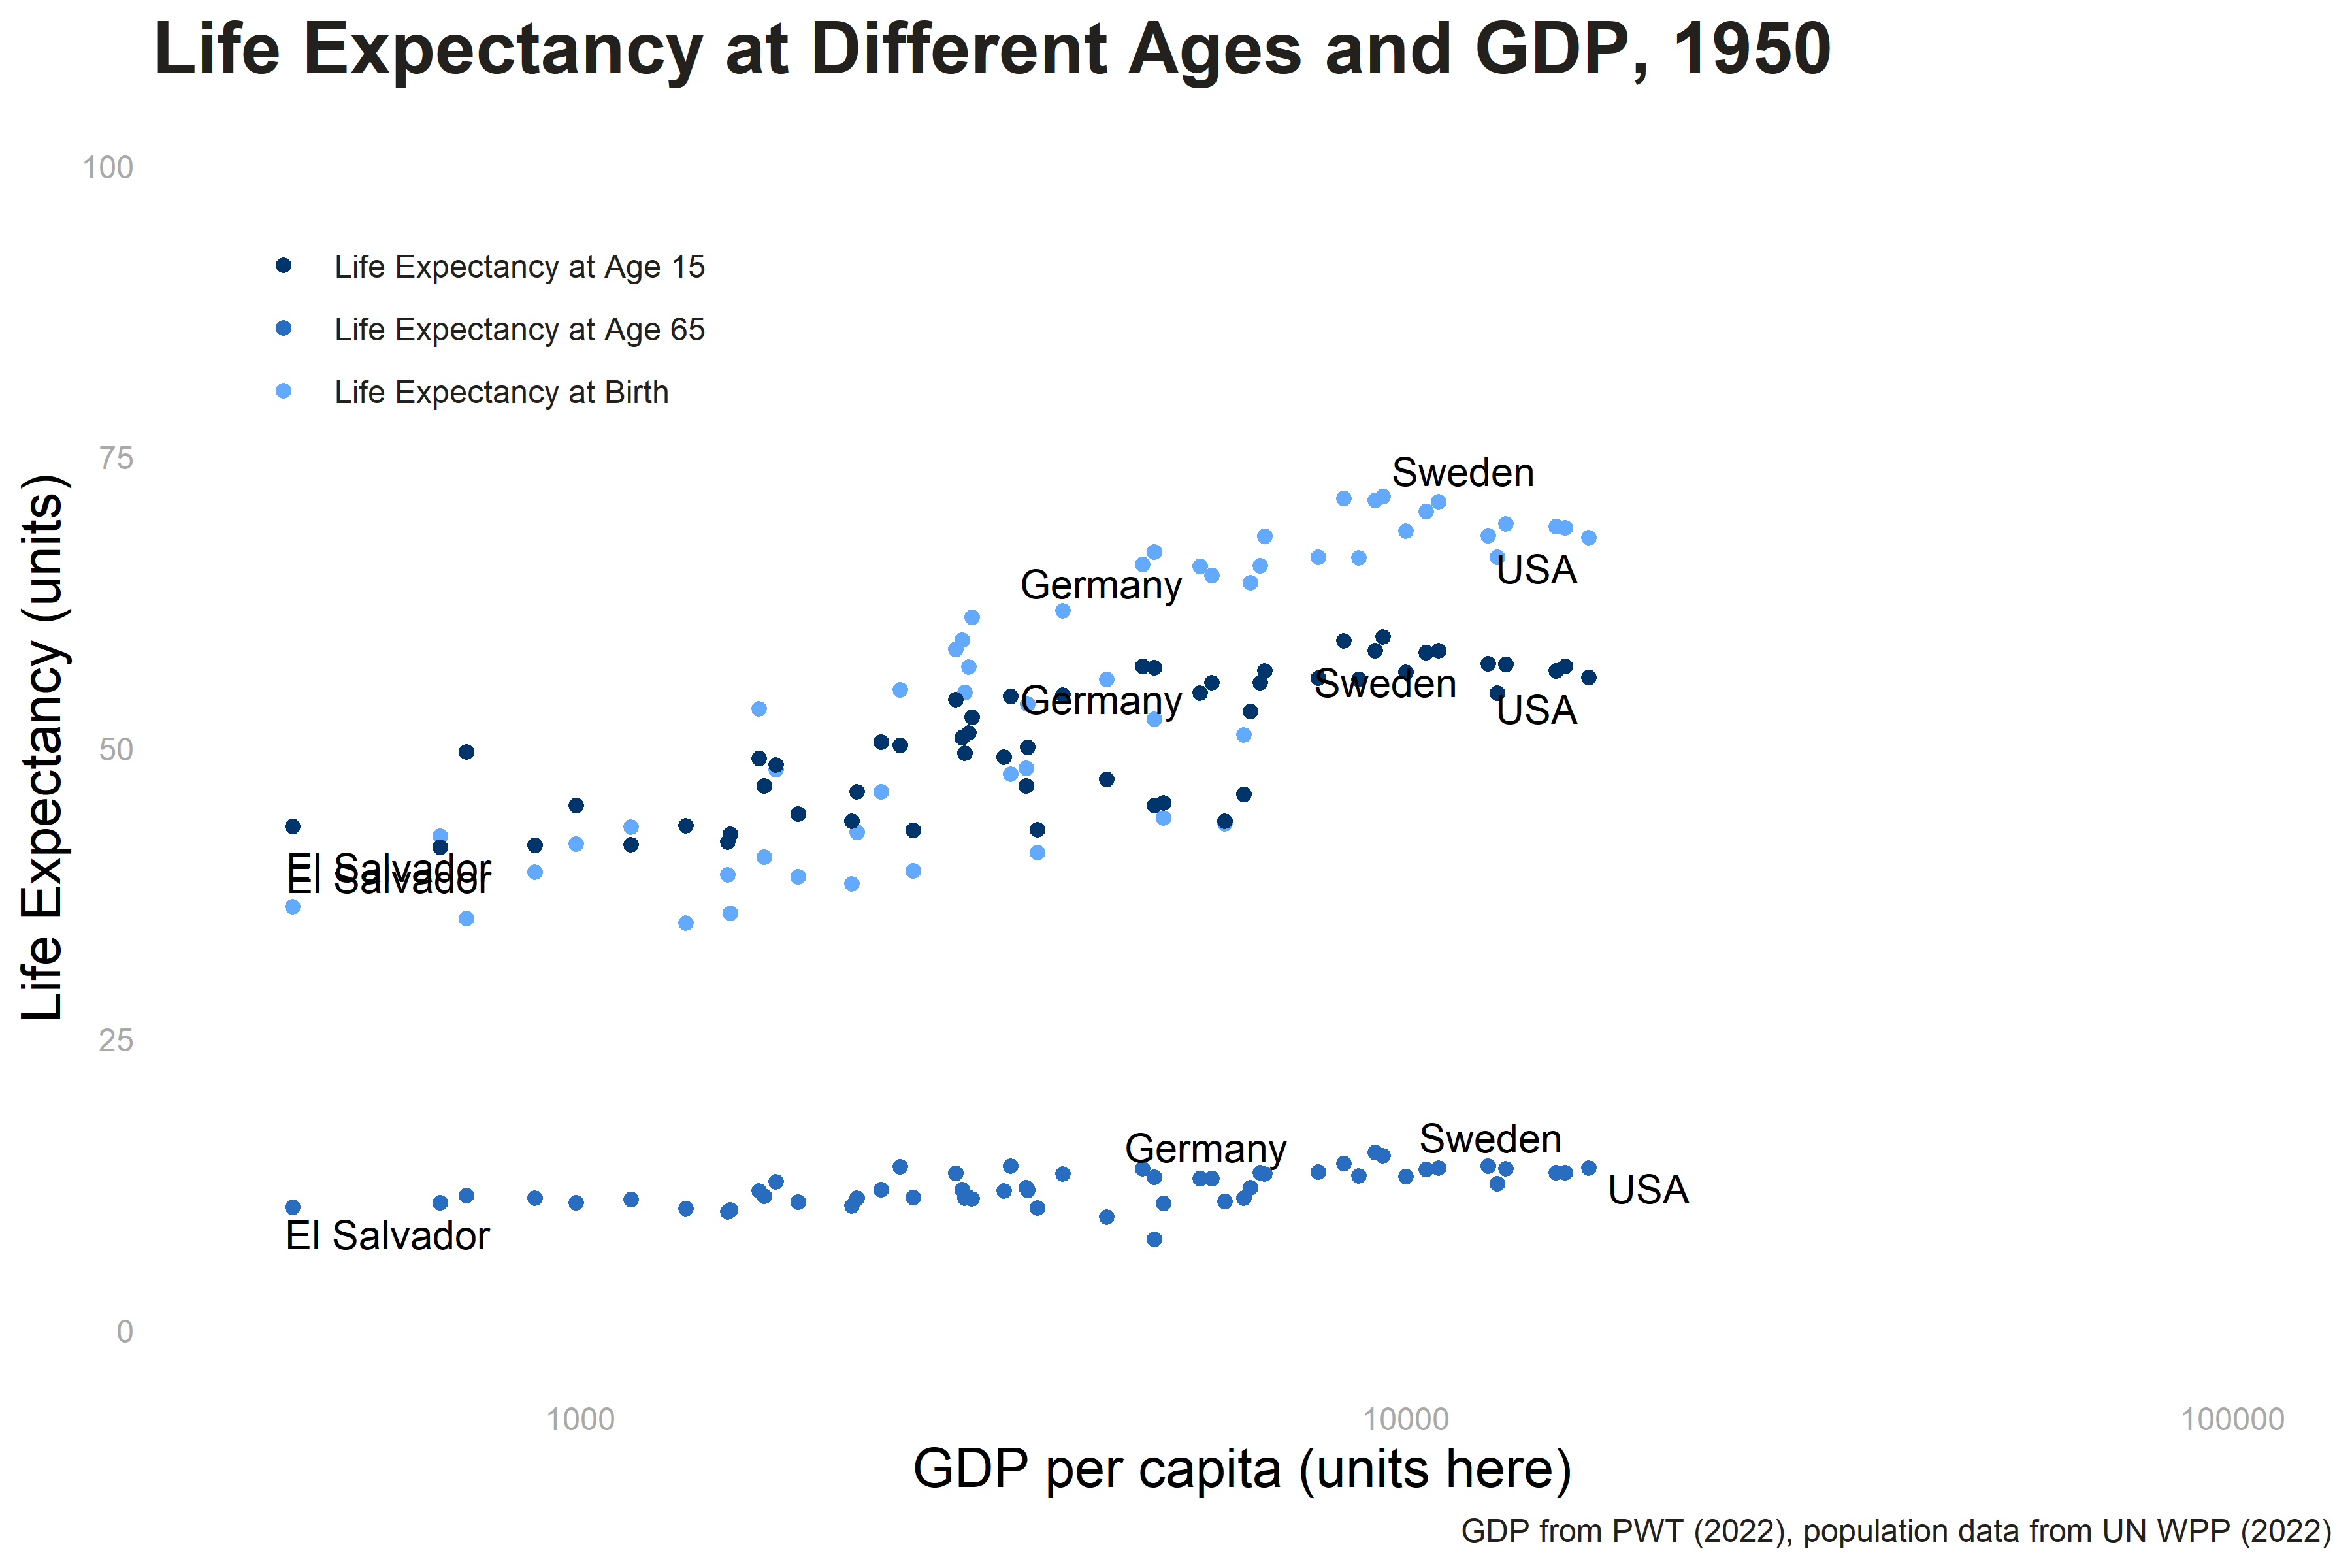
\includegraphics[width=\textwidth]{figures/ECON-412/gdp_pc_le_1950.png}
  \caption{1971}
  \label{fig:sub1}
\end{subfigure}%
\begin{subfigure}[h]{0.5\textwidth}
  \centering
  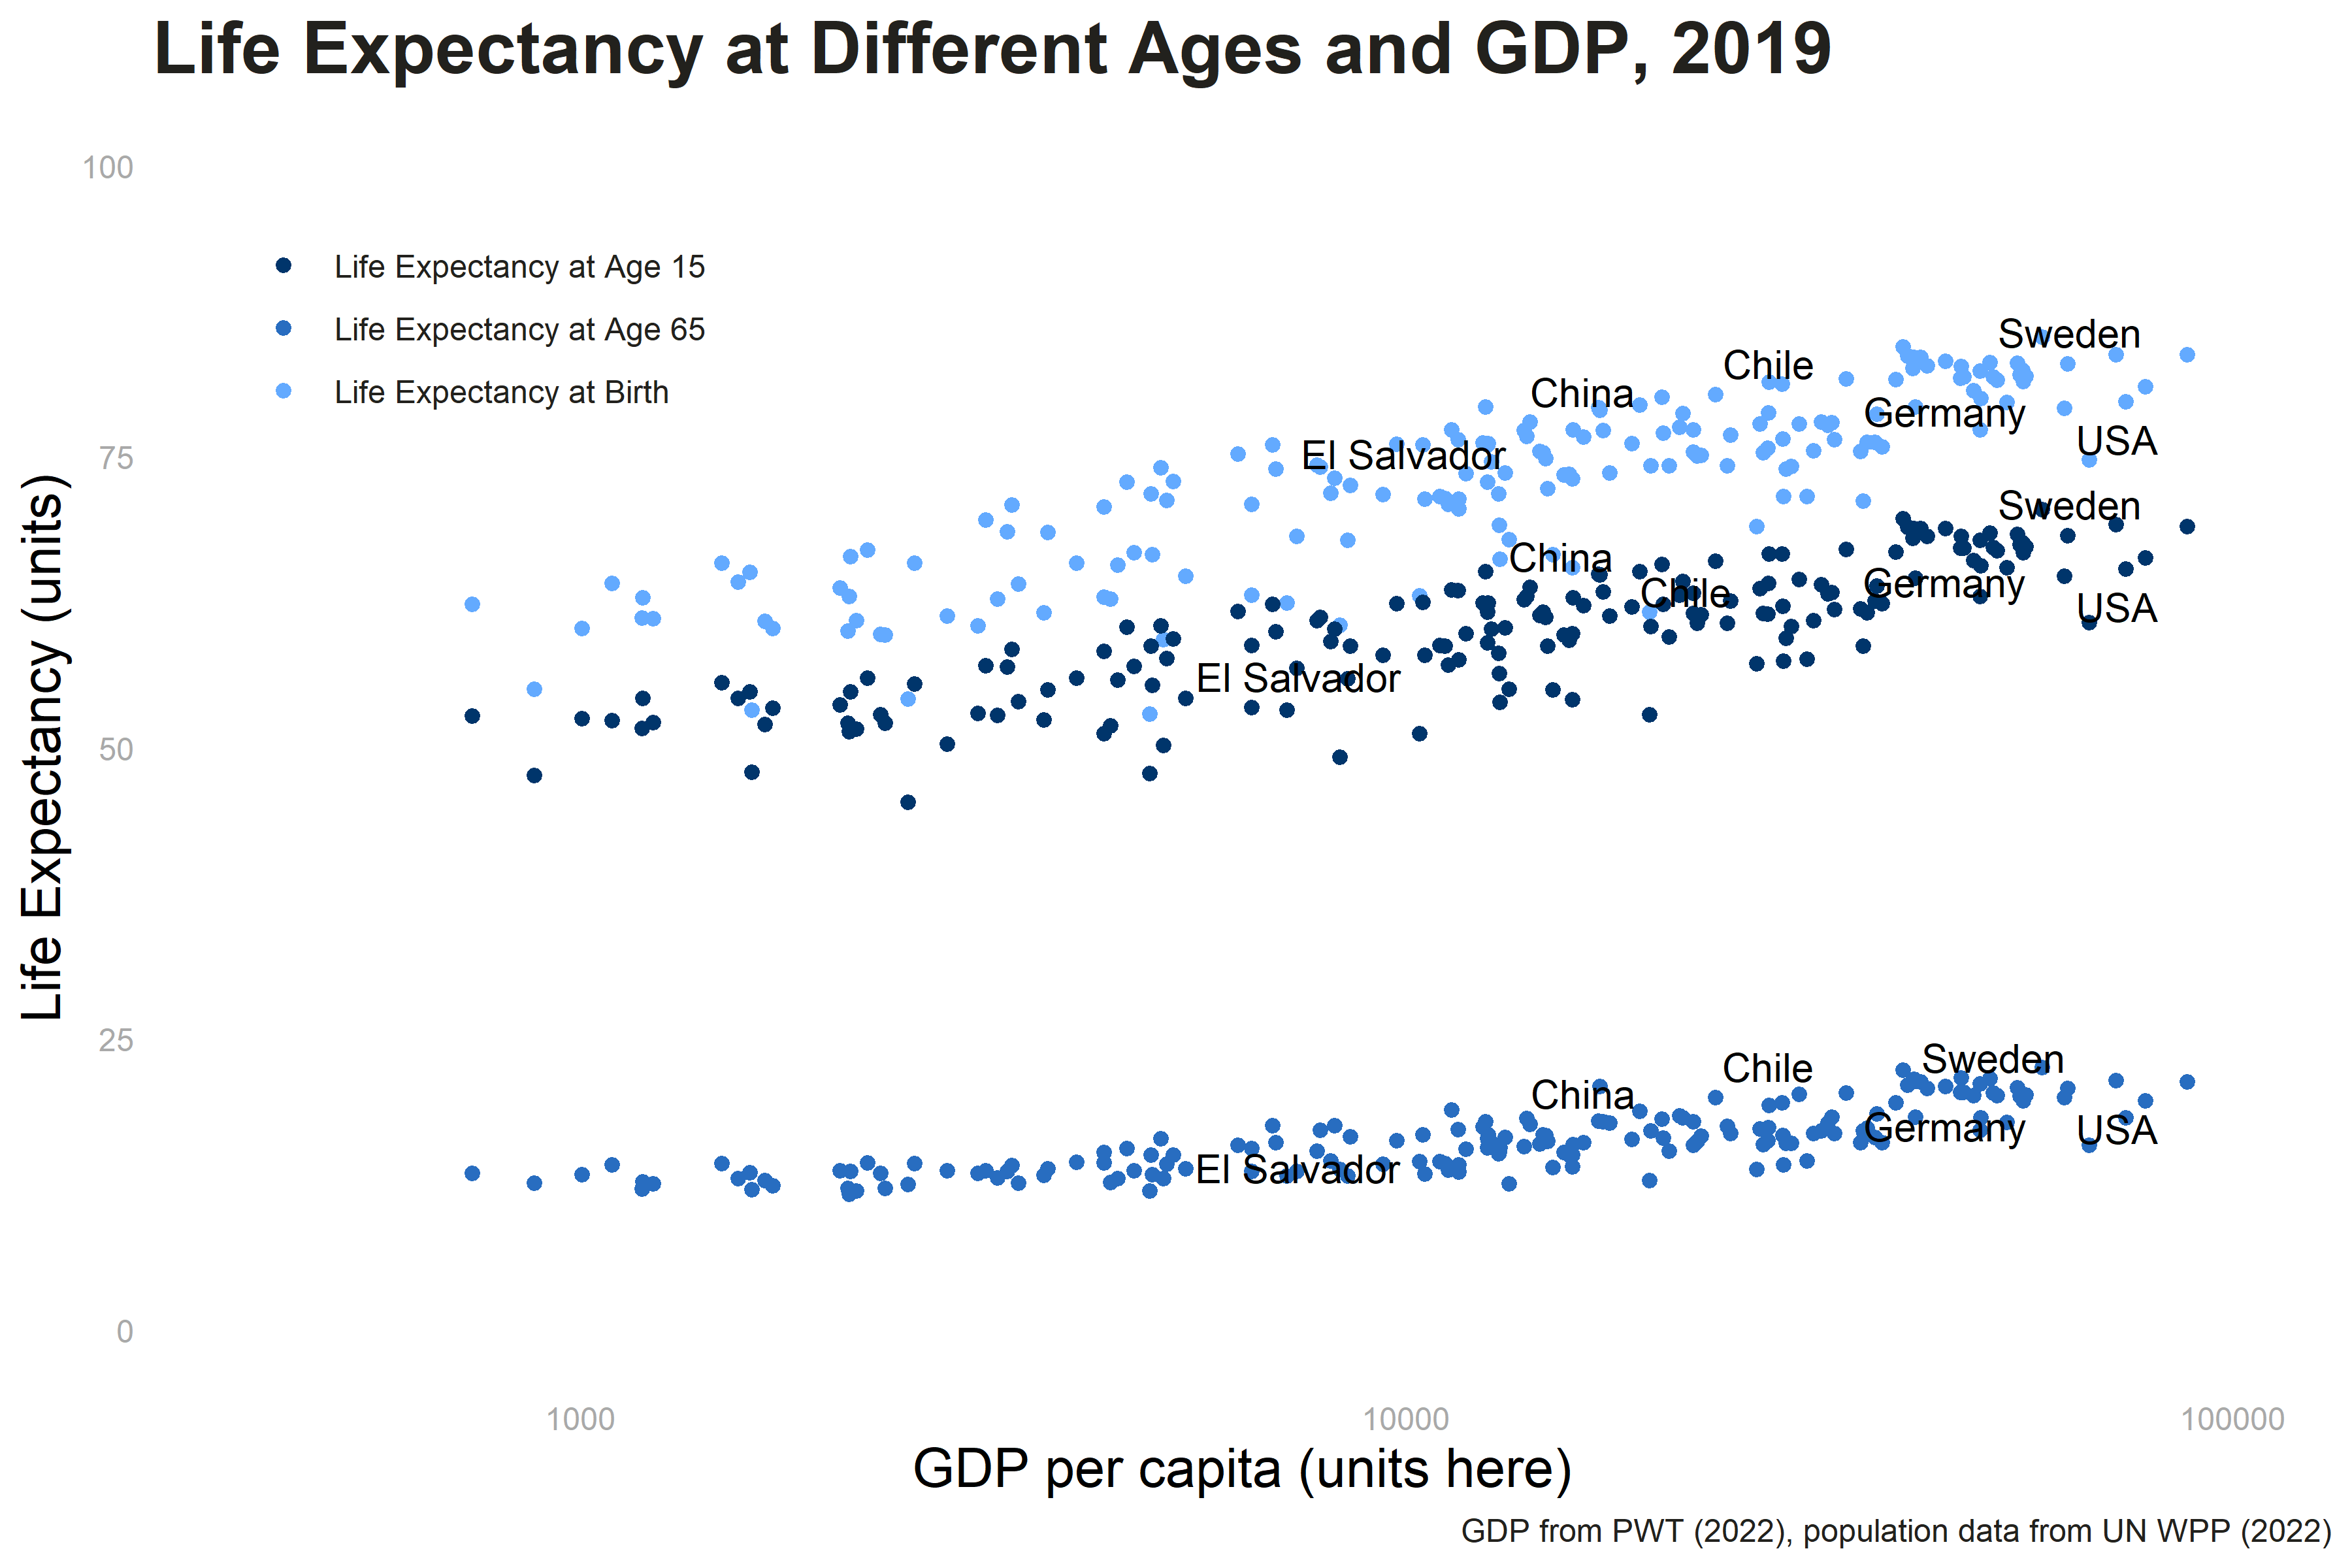
\includegraphics[width=\textwidth]{figures/ECON-412/gdp_pc_le_2019.png}
  \caption{2019}
  \label{fig:sub2}
\end{subfigure}
\caption{Comparison of Life Expectancies to GDP per capita over time}
\label{fig:fig_01}
\end{figure}

\begin{figure}[H]
	\centering % centers
	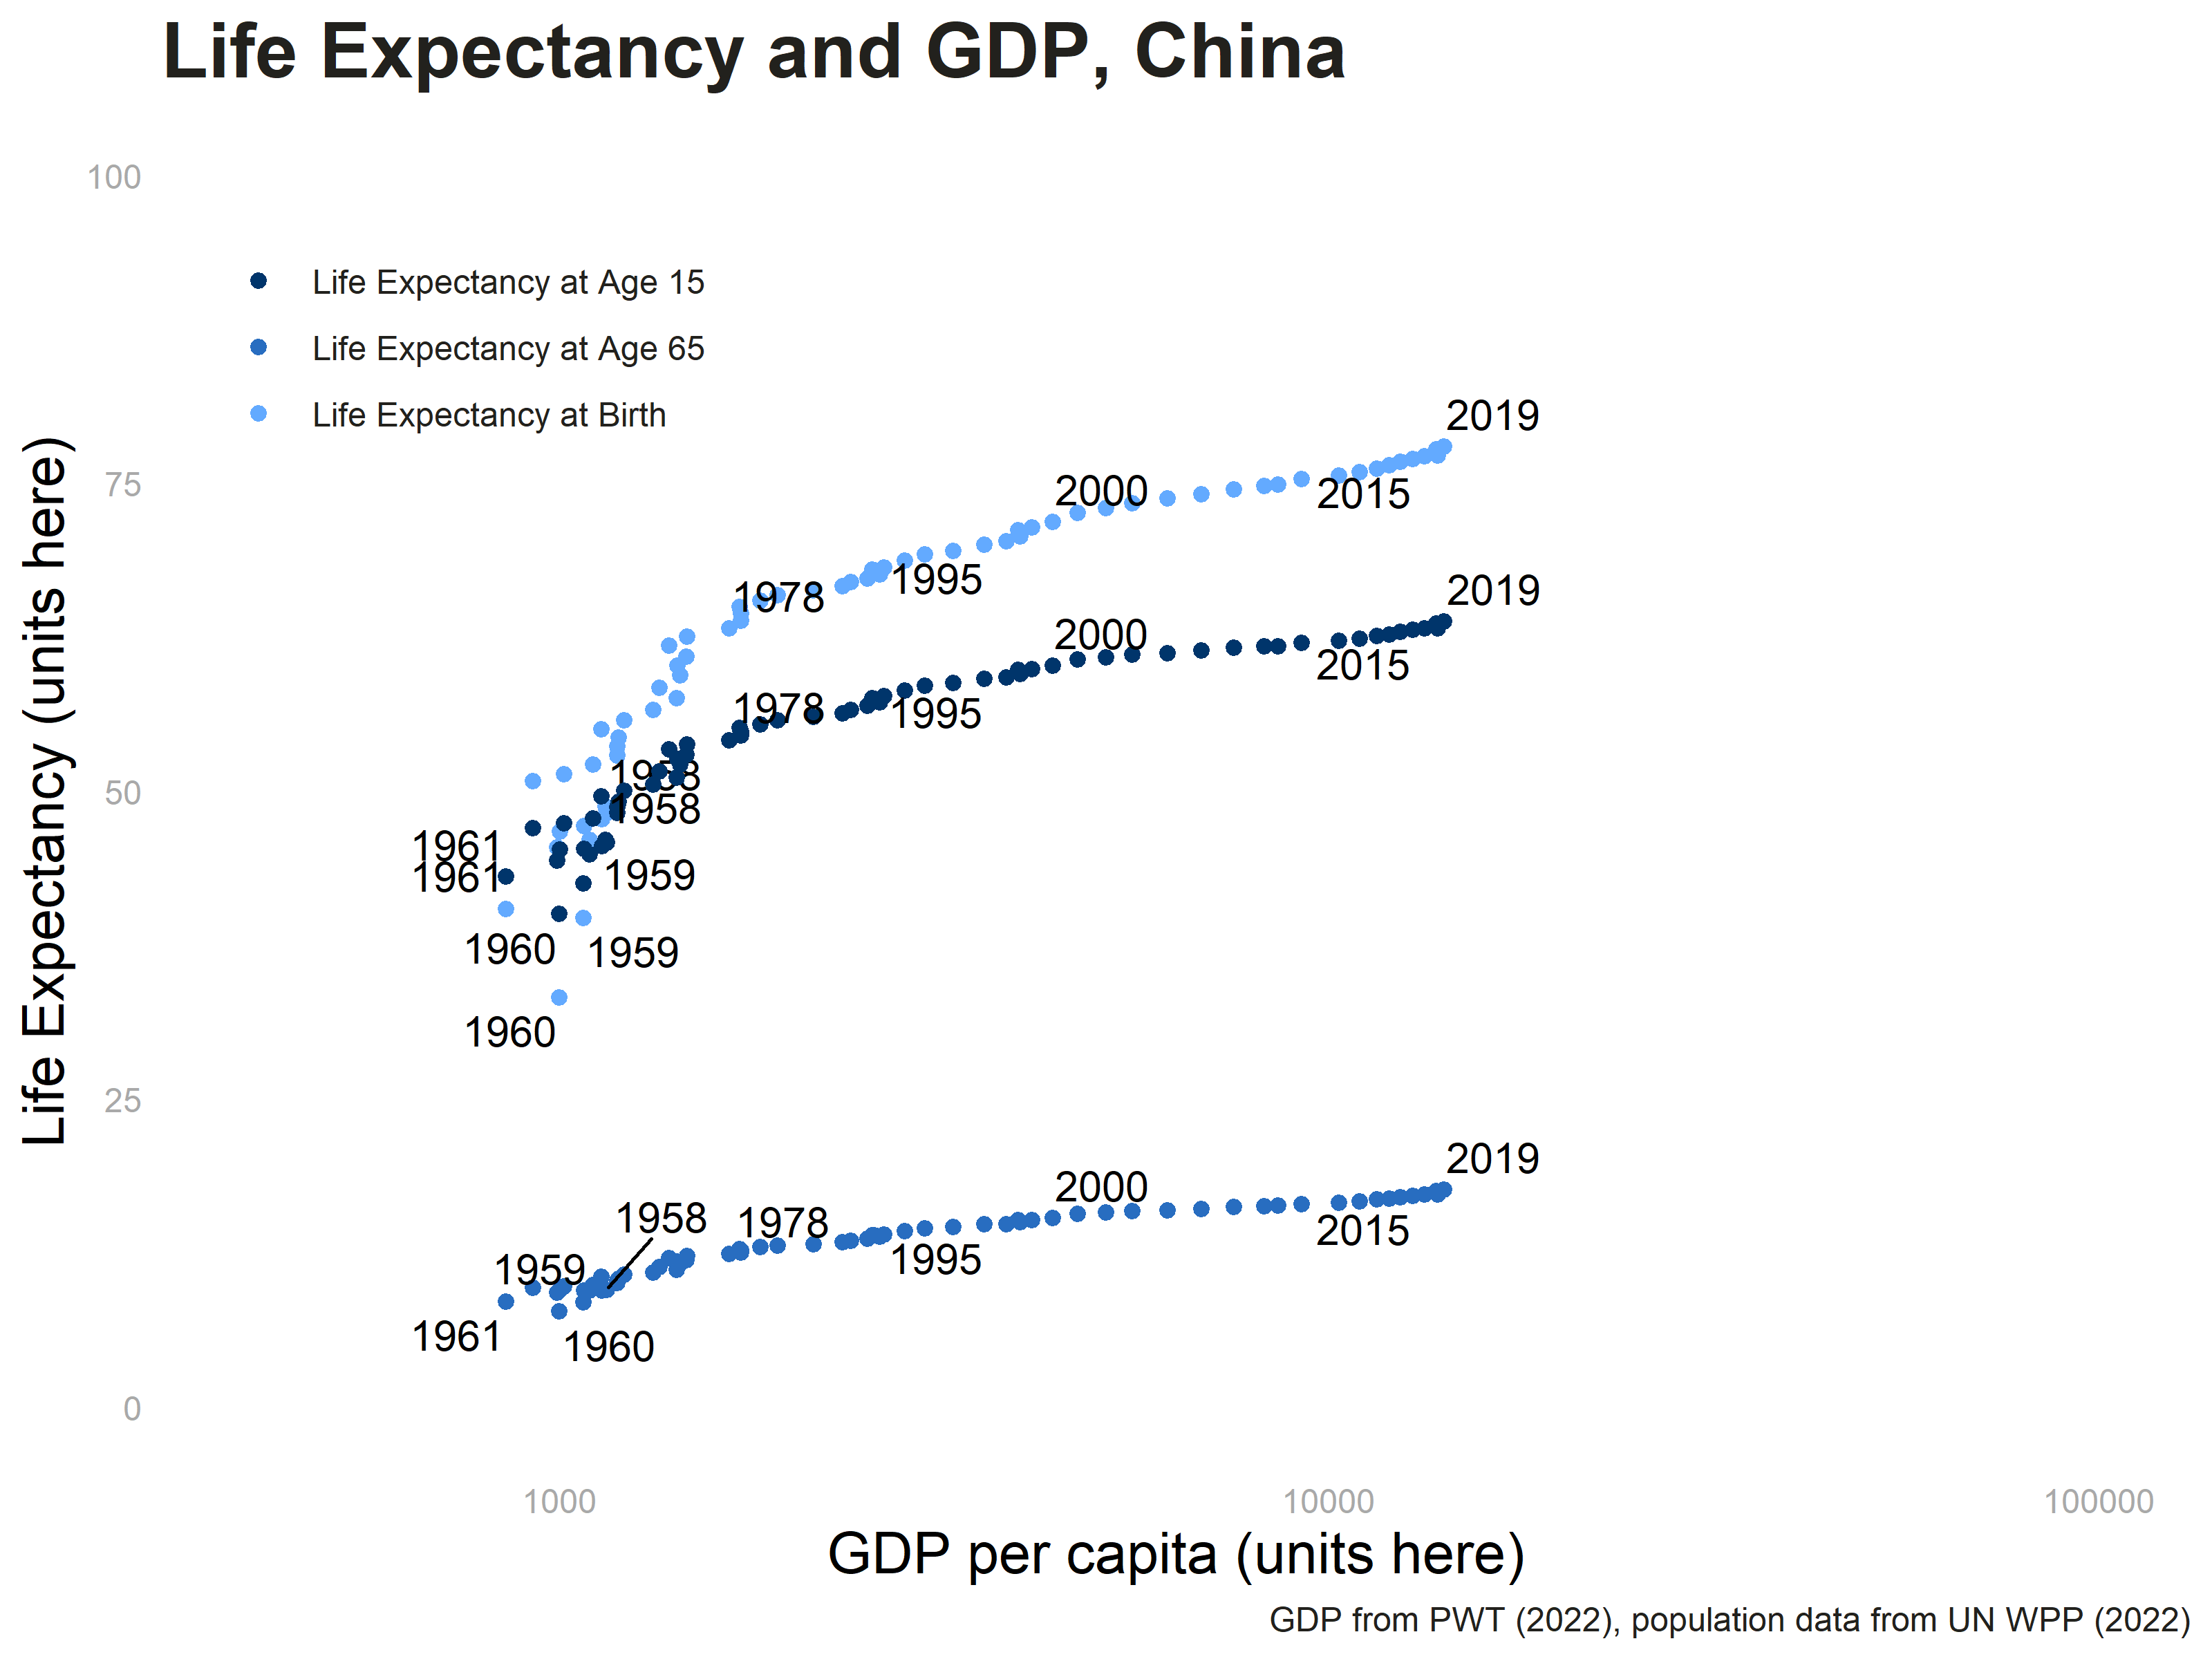
\includegraphics[width=.6\linewidth]{figures/ECON-412/gdp_pc_le_China.png}
	\caption{China's Evolution, 1950-2019} % note caption is required in order to get the cross referencing
	\label{fig:fig3}
\end{figure}



\subsection{Results}

Now let's run some regressions and generate some predictions.


\begin{enumerate}
    \item Adapt your code in \verb+code/03_analysis/03_analysis_hw-03.R+ to generate two tables that correspond to Equations 1 through 5 above. One of these tables should include the results of running regressions from Equations 1 through 3 on the same two years you showed for your figures in Figure~\ref{fig:fig_01}. The code will be similar to that which generated Table~\ref{tab:lecrosssection}. 
    \item The other table should include the results from Equation~\ref{eq:eq_4} and Equation~\ref{eq:eq_5}, with the regression for Equation~\ref{eq:eq_4} restricted to the most recent year, and Equation~\ref{eq:eq_5} a panel over multiple available years. You may find it useful to adapt the code which produced Table~\ref{tab:lepanelregs}.\footnote{It's your choice whether you'd like to restrict the data to a balanced panel, i.e. where all years and all units are available, or whether you'd like to use an unbalanced panel in which you include whatever country-year combinations are available. But whichever you do, spend a couple minutes to think about what the trade-offs are.}
    \item Interpret the results for each column of each table in words (no need to be repetitive, but make clear the distinctions between them). Describe the economic and statistical significance of these coefficients. What is your preferred specification and why? Are any of these results surprising or otherwise noteworthy? 
    \item Adapt the code of \verb+code/04_plots/04_plots_hw-03_template.R+ to generate a scatter plot with GDP per capita on the X axis, and predicted values for greenhouse gas emissions per capita on the Y axis, according to the specification of Equation~\ref{eq:eq_5}. This corresponds fairly closely to the exercise of \citet{grossmanEconomicGrowthEnvironment1995}, yielding a plot like Figure~\ref{fig:fig4}. Do you observe an environmental Kuznets curve? Comment on why or why not. Has your analysis made a causal argument? Comment on why or why not.
\end{enumerate}

\begin{figure}[H]
	\centering % centers
	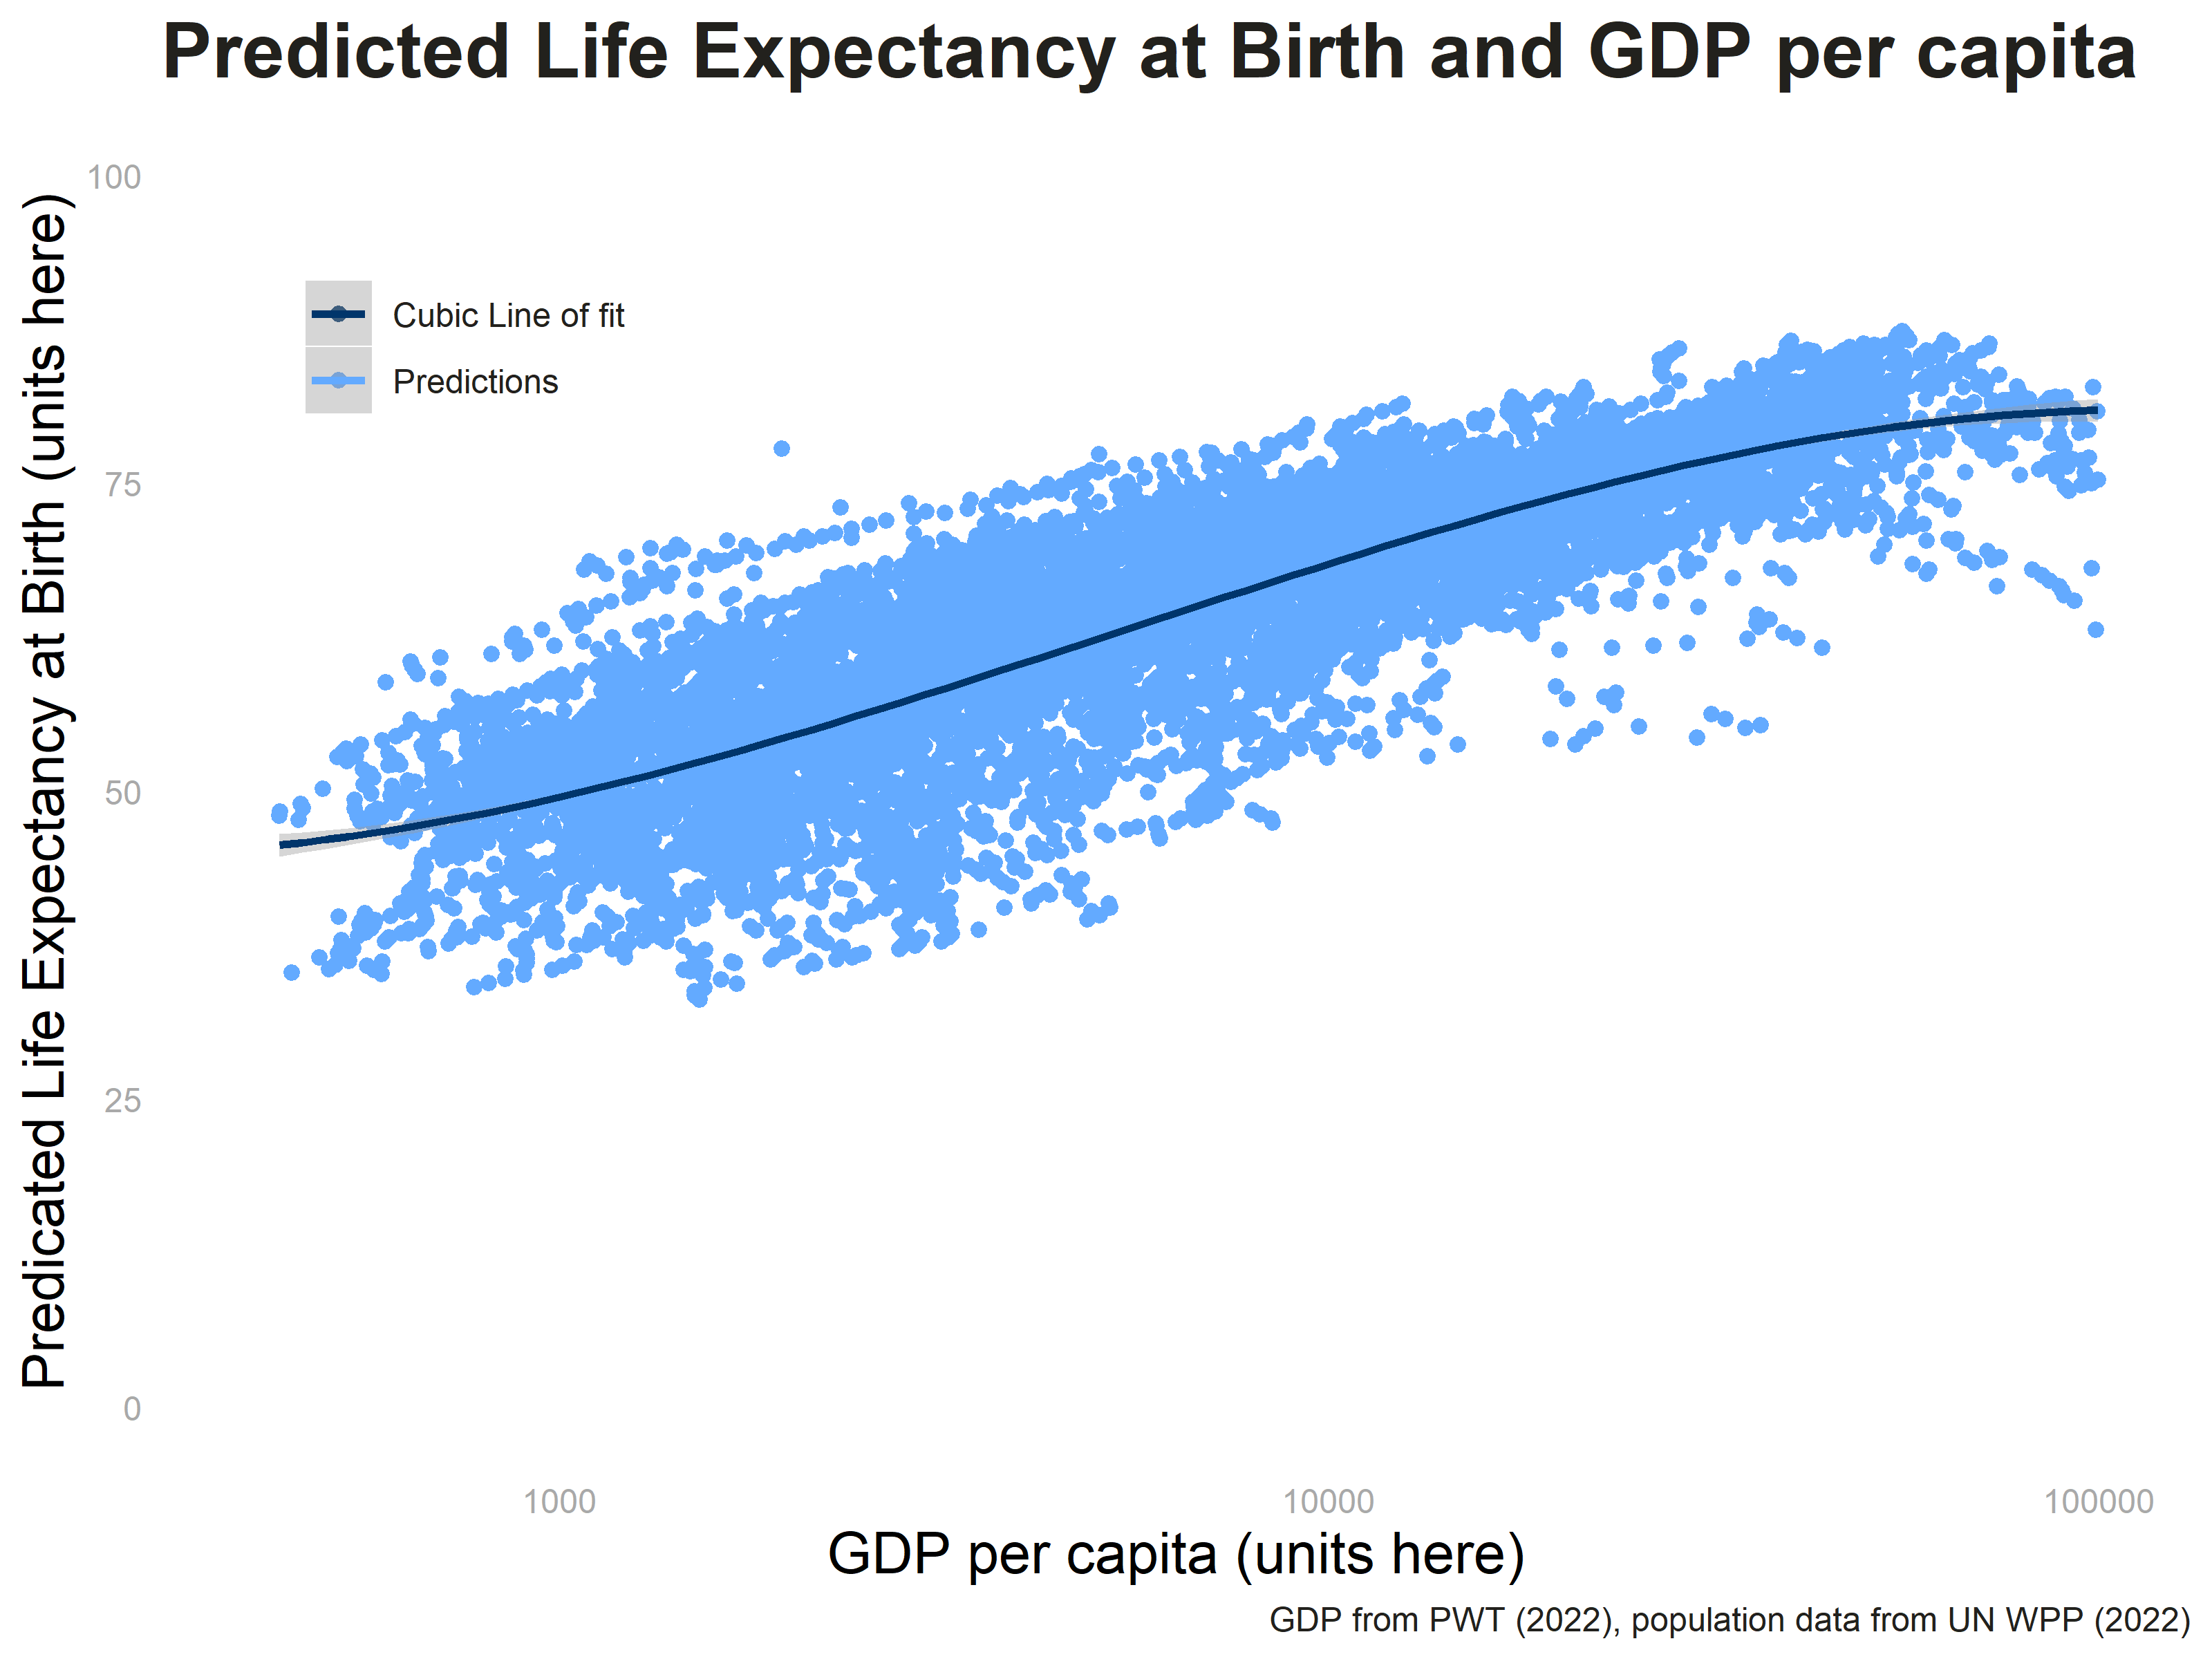
\includegraphics[width=.6\linewidth]{figures/ECON-412/gdp_pc_le_predictions.png}
	\caption{Predicted Values} % note caption is required in order to get the cross referencing
	\label{fig:fig4}
\end{figure}

\begin{comment}

\begin{figure}[H]
	\centering % centers
	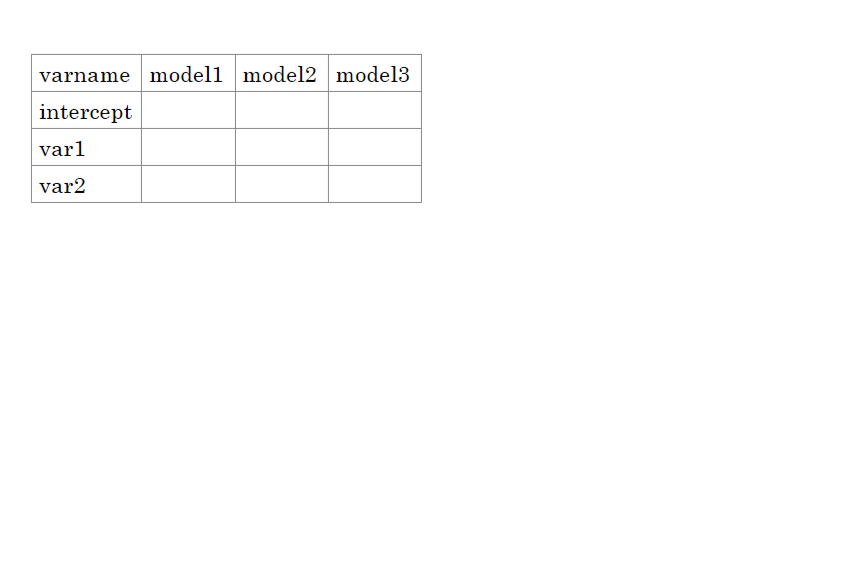
\includegraphics[width=.6\linewidth]{figures/ECON-412/hw-03_table1.png}
	\caption{Example Screenshot for Table Requirement} % note caption is required in order to get the cross referencing
	\label{fig:fig4}
\end{figure}

\end{comment}



% note this requires
%\usepackage{threeparttablex} in the preamble

\begin{table}[H]

\caption{Life Expectancy Cross-Section Comparisons, 1950 and 2019 \label{tab:lecrosssection}}
\centering
\begin{threeparttable}
\begin{tabular}[t]{lcccccc}
\toprule
\multicolumn{1}{c}{ } & \multicolumn{2}{c}{Birth} & \multicolumn{2}{c}{Age 15} & \multicolumn{2}{c}{Age 65} \\
\cmidrule(l{3pt}r{3pt}){2-3} \cmidrule(l{3pt}r{3pt}){4-5} \cmidrule(l{3pt}r{3pt}){6-7}
\multicolumn{1}{c}{ } & \multicolumn{1}{c}{1950} & \multicolumn{1}{c}{2019} & \multicolumn{1}{c}{1950} & \multicolumn{1}{c}{2019} & \multicolumn{1}{c}{1950} & \multicolumn{1}{c}{2019} \\
\cmidrule(l{3pt}r{3pt}){2-2} \cmidrule(l{3pt}r{3pt}){3-3} \cmidrule(l{3pt}r{3pt}){4-4} \cmidrule(l{3pt}r{3pt}){5-5} \cmidrule(l{3pt}r{3pt}){6-6} \cmidrule(l{3pt}r{3pt}){7-7}
  & (1) & (2) & (3) & (4) & (5) & (6)\\
\midrule
Intercept & 42.823 & 67.733 & 42.617 & 42.102 & 11.127 & 14.266\\
 & (1.676) & (0.665) & (6.361) & (4.614) & (0.224) & (0.201)\\
GDP per capita & 0.002 & 0.000 &  &  &  & \\
 & (0.000) & (0.000) &  &  &  & \\
Log GDP per capita &  &  & 2.073 & 2.359 &  & \\
 &  &  & (0.651) & (0.401) &  & \\
TFR &  &  & -1.880 & -1.671 &  & \\
 &  &  & (0.288) & (0.363) &  & \\
GDP (unit) per (unit) &  &  &  &  & 0.213 & 0.093\\
 &  &  &  &  & (0.028) & (0.009)\\
\midrule
Num.Obs. & 55 & 182 & 55 & 182 & 55 & 182\\
Mean & 54.870 & 73.080 & 50.660 & 60.220 & 12.260 & 16.370\\
R2 & 0.611 & 0.508 & 0.769 & 0.724 & 0.360 & 0.572\\
R2 Adj. & 0.604 & 0.505 & 0.760 & 0.721 & 0.348 & 0.569\\
F & 78.666 & 98.508 & 88.414 & 209.054 & 56.186 & 108.220\\
\bottomrule
\end{tabular}
\begin{tablenotes}
\item \textit{Notes: } 
\item Robust standard errors given in parentheses. Population and life expectancy are obtained from \citet{undesaWorldPopulationProspects2022}. Gross domestic product (GDP) is (what units) from \citet{feenstraNextGenerationPenn2015}.
\end{tablenotes}
\end{threeparttable}
\end{table}

\begin{table}[H]

\caption{Panel Regression, Life Expectancy \label{tab:lepanelregs}}
\centering
\begin{threeparttable}
\begin{tabular}[t]{lcccc}
\toprule
\multicolumn{1}{c}{ } & \multicolumn{4}{c}{Life Expectancy at Birth} \\
\cmidrule(l{3pt}r{3pt}){2-5}
\multicolumn{1}{c}{ } & \multicolumn{1}{c}{1950} & \multicolumn{1}{c}{2019} & \multicolumn{1}{c}{Within} & \multicolumn{1}{c}{Twoway} \\
\cmidrule(l{3pt}r{3pt}){2-2} \cmidrule(l{3pt}r{3pt}){3-3} \cmidrule(l{3pt}r{3pt}){4-4} \cmidrule(l{3pt}r{3pt}){5-5}
  & (1) & (2) & (3) & (4)\\
\midrule
Intercept & 33.437 & 62.576 &  & \\
 & (2.405) & (0.789) &  & \\
GDP (units) per (units) capita & 6.714 & 0.891 & 0.821 & -0.141\\
 & (1.609) & (0.082) & (0.065) & (0.048)\\
(GDP(units) per (units))$$^2$$ & -0.373 & -0.014 & -0.008 & 0.001\\
 & (0.217) & (0.002) & (0.001) & (0.000)\\
(GDP (units) per (units))$$^3$$ & 0.006 & 0.000 & 0.000 & 0.000\\
 & (0.008) & (0.000) & (0.000) & (0.000)\\
\midrule
Mean & 54.87 & 73.08 & 64.31 & 64.31\\
Country FE & N & N & Y & Y\\
Time FE & N & N & N & Y\\
Num.Obs. & 55 & 182 & 10201 & 10201\\
R2 & 0.743 & 0.694 & 0.785 & 0.929\\
R2 Within &  &  & 0.302 & 0.035\\
\bottomrule
\end{tabular}
\begin{tablenotes}
\item \textit{Notes: } 
\item Heteroskedascicity-robust standard errors clustered at the country (for within) and country and year (for twoways) levels given in parentheses. Population and life expectancy data are from \citet{undesaWorldPopulationProspects2022}. Gross domestic product (GDP) is (what units) from \citet{feenstraNextGenerationPenn2015}.
\end{tablenotes}
\end{threeparttable}
\end{table}




